\section{Theorie}\label{theorie}
\subsection{Eigenschaften idealer Operationsverstärker}
Soll Verständnis über die Funktionsweise von Operationsverstärkern erlangt werden, so kann es helfen, diese auf ein paar ideale Eigenschaften zu beschränken. Werden mit diesen Annahmen Berechnungen durchgeführt, fallen im Regelfall nur geringe Abweichungen auf und die reduzierten Rechenregeln können als überzeugende Grundlage verwendet werden.
Im Generellen kann gesagt werden, dass ein Operationsverstärker als gleichstromgekoppelter Differenzverstärker arbeitet.
Ein unbeschalteter Aufbau eines Operationsverstärkers ist in Abbildung \ref{unbeschaltet} zu sehen.

\begin{figure}[H]
  \centering
  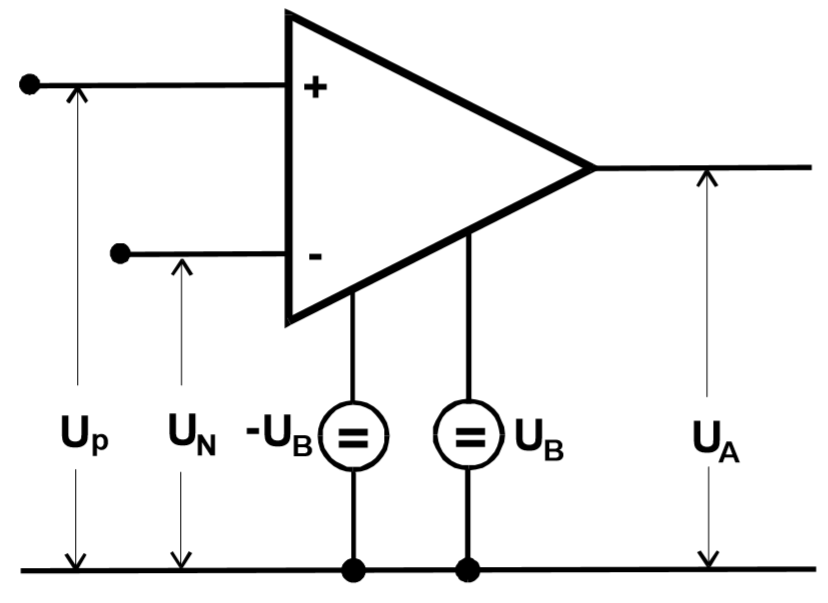
\includegraphics[width=0.45\textwidth]{bilder/unbeschaltet.png}
  \caption{Schematische Darstellung eines Operationsverstärkers mit Einzeichnung der Anschlussgrößen \cite{anleitung}.}
  \label{unbeschaltet}
\end{figure}

Zu erkennen ist, dass ein jener über einen invertierenden~$(-)$  und einen nicht-invertierenden $(+)$  Anschluss verfügt, über den eine Besteuerung erfolgt. Diesen gefolgt ist ein Ausgang $U_\text{A}$, über den das Ausgangssignal abgegriffen werden kann.
Im Idealfall gilt eine Proportionalität $V$ zwischen der Differenz der beiden Eingangssignale $U_-$ und $U_+$ und dem resultierenden Ausgangssignal:
\begin{equation}
  U_\text{A}=V(U_+-U_-)\,.
\end{equation}
Dieser Zusammenhang ist für einen realen Operationsverstärker, abgesehen von im Experiment auftretbaren Überschwingern, alleinig innerhalb des Aussteuerungsbereichs des Verstärkers gültig. Dieser ist durch die, wie in Abbildung \ref{unbeschaltet} zu sehen ist, angelegte Betriebsspannung $\pm U_\text{B}$ festgelegt und nur innerhalb dieses Bereichs kann eine Verstärkung $V$ des Eingangssignals erfolgen. Übersteigt das Ausgangssignal in seiner Größe diesen Wertebereich, folgt ein konstanter Wert $U_\text{B}$ am Ausgang.
Es gilt somit
\begin{equation}
  -U_\text{B} < U_\text{A} < +U_\text{B}\,.
\end{equation}
Grafisch ergibt sich die in Abbildung \ref{kennlinie} dargestellte Kennlinie.

\begin{figure}[H]
  \centering
  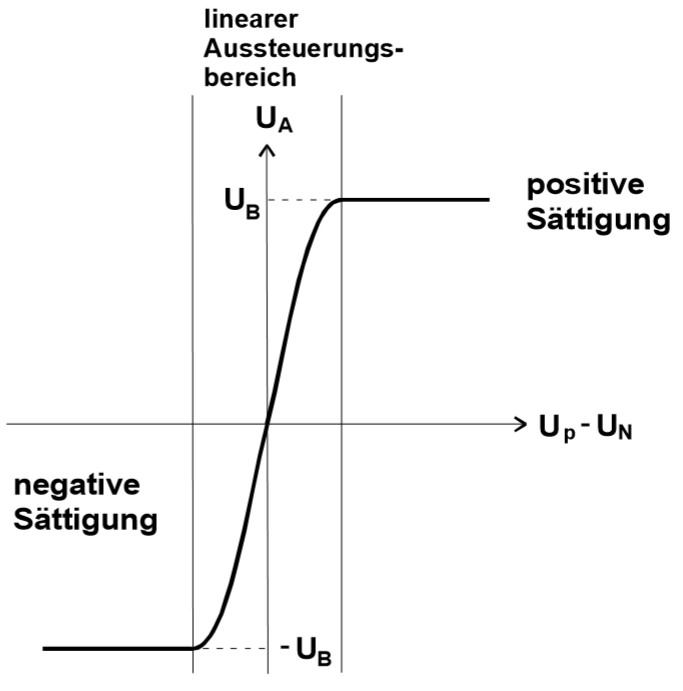
\includegraphics[width=0.45\textwidth]{bilder/kennlinie.png}
  \caption{Typische Kennlinie eines realen Operationsverstärkers mit dem linearen Verhalten innerhalb des Ansteuerungsbereichs \cite{anleitung}.}
  \label{kennlinie}
\end{figure}

Im Folgenden wird auf die wichtigsten Kenngrößen idealer Operationsverstärker eingegangen.
Das primäre Ziel eines jenen ist das Erreichen einer möglichst großen Verstärkung. Ideal sollte diese gegen $\infty$ gehen.
Die differentiellen Widerstände für Eingang und Ausgang liegen auch in ihren Grenzwerten beschrieben.
Idealerweise liegt der Eingangswiderstand im Unendlichen; der Ausgangswiderstand beeinflusst das Signal kaum und sollte möglichst den Wert Null annehmen.
Hieraus folgen die wichtigsten Regeln für Berechnungen von Operationsverstärkerbeschaltungen:
\begin{align*}
1.\quad& \text{Nach Möglichkeit Verstärkung bis ins Unendliche:}\\
&\quad V=\infty\\
2.\quad& \text{Die Differenz der Eingangsspannungen ist Null:}\\
&\quad U_\text{D}=U_+-U_-=0\\
3.\quad& \text{Die Eingangsströme sind gleich Null:}\\
&\quad I_+=I_-=0\,.
\end{align*}
\subsection{Überleitung zu realem Verhalten von Operationsverstärkern}
Werden reale Operationsverstärker betrachtet, so wird sich für weitere Kenngrößen interessiert.
Eine charakteristische Kenngröße ist die Gleichtaktverstärkung
\begin{equation}
V_\text{Gl}=\frac{\text{\Delta}U_\text{A}}{\text{\Delta}U_\text{Gl}}\,,
\end{equation}
mit einer selben Spannung $U_\text{Gl}$ an beiden Eingängen.
Wird an den beiden Eingängen dieselbe Spannung angelegt, so würde bei einem idealen Operationsverstärker $U_A=0$ folgen.
Bei einem realen Operationsverstärker ist demnach die Gleichtaktverstärkung ein Maß für die Verzerrung innerhalb des Verstärkerbauteils.\\
Da reale Operationsverstärker endliche Eingangsströme besitzen, wird der Eingangsruhestrom
\begin{equation}
I_\text{B}=\frac{1}{2}(I_\text{p}+I_\text{N})
\end{equation}
definiert.
Des Weiteren folgt die Definition des Offsetstroms
\begin{equation}
I_0=I_\text{p}-I_\text{N}\quad \text{bei}\quad U_\text{p}=U_\text{N}=0\,.
\end{equation}
Darüberhinaus folgen die Definitionen des Gleichtakteingangswiderstands
\begin{equation}
  r_\text{Gl}=\frac{\text{\Delta}U_\text{Gl}}{\text{\Delta}I_\text{Gl}}\quad\text{mit}\quad U_\text{Gl}=U_\text{p}=U_\text{N}\quad\text{und}\quad I_\text{Gl}=I_\text{p}+I_\text{N}
\end{equation}
und der Offsetspannung
\begin{equation*}
  U_0=U_\text{p}-U_\text{N}\quad\text{für}\;U_\text{A}=0\,.
\end{equation*}


\subsection{Schaltungen mit Operationsverstärkern}
In den folgenden Unterkapiteln werden weiterführende Beschaltungen eines Operationsverstärkers betrachtet. Es handelt sich um Standard-Beschaltungen, die einfache Rechenoperationen darstellen können.
\subsubsection{Invertierender Verstärker}
  Bei einem invertierenden Verstärker, auch Linearverstärker genannt, wird mit einer Gegenkopplung gearbeitet. Dies beschreibt das Rückführen des Ausgangssignals auf den invertierenden Eingang, was zum Ziel hat, eine Dämpfung zu erzeugen und Verzerrungen im Ausgangssignal entgegenzuwirken.
  Ein Schaltbeispiel ist in Abbildung \ref{invert} zu sehen.

  \begin{figure}[H]
    \centering
    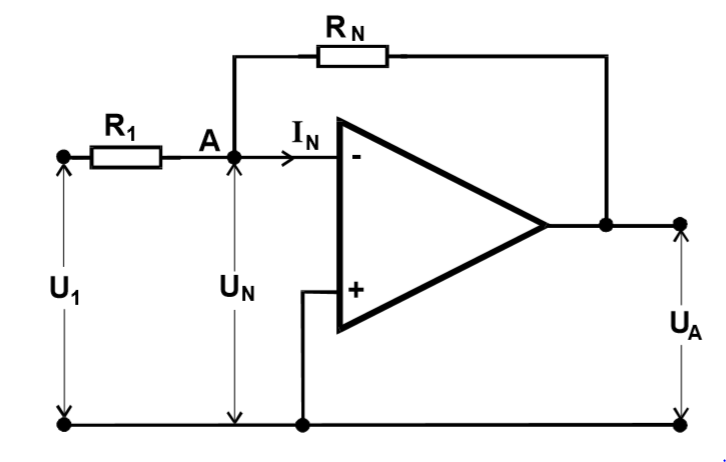
\includegraphics[width=0.45\textwidth]{bilder/invert.png}
    \caption{Schematische Darstellung eines invertierenden Verstärkers mit den Gegenkopplungswiderständen $R_1$ und $R_\text{N}$ \cite{anleitung}.}
    \label{invert}
  \end{figure}

Aufgrund der sehr großen Leerlaufverstärkung wird $U_\text{N}=0$ angenommen und mithilfe der Kirchhoffschen Regeln kann der folgende Zusammenhang aufgestellt werden:
\begin{equation}
  \frac{U_1}{R_1}+\frac{U_\text{A}}{R_\text{N}}=0\,.
\end{equation}
  Somit kann eine Relation für die reale Leerlaufverstärkung $V'$ hergeleitet werden:
  \begin{equation}
    V'=\frac{U_\text{A}}{U_\text{1}}=-\frac{R_\text{N}}{R_1}\,.
    \label{eq:V_linear}
  \end{equation}
  Die Widerstände $R_1$ und $R_\text{N}$ bedienen die Gegenkopplung. Für reale Operationsverstärker muss eine endliche Leerlaufverstärkung angenommen werden. Es lässt sich
  \begin{equation}
    U_\text{N}=-\frac{U_\text{A}}{V}
  \end{equation}
  folgern.
  Mit der Annahme $I_\text{N}=0$ kann daraus für den Knotenpunkt A die Relation
  \begin{equation}
    \frac{U_\text{N}-U_1}{U_\text{A}-U_1}=\frac{R_1}{R_1+R_\text{N}}
  \end{equation}
  hergeleitet werden. Über das Verhältnis von $U_\text{A}$ zu $U_1$ folgt
  \begin{equation}
    \frac{1}{V'}=\frac{1}{V}+\frac{R_1}{R_\text{N}}\,.
  \end{equation}
  Wird die Verstärkung in Abhängigkeit der Frequenz des Eingangssignals betrachtet, so ist auffällig, dass die Verstärkung nicht im Betrag linear mit der Frequenz anwächst. Vielmehr muss insbesondere für einen Linearverstärker die Frequenzabhängigkeit untersucht werden. Es zeigt sich oft ein Verhalten, wie es Abbildung \ref{abb:bandbreite} zeigt.
  Die Bandbreite ist der Begriff für das Frequenzintervall, in dem die Verstärkung auf den Faktor $\frac{1}{\sqrt{2}}$ abgefallen ist. Diese Frequenz wird Grenzfrequenz $\nu_\text{Grenz}$ genannt. Für den weiteren Text wird die Verstärkung in ihrem Maximalwert vor dem Abfall mit $V_0$ bezeichnet.
  \begin{figure}[H]
    \centering
    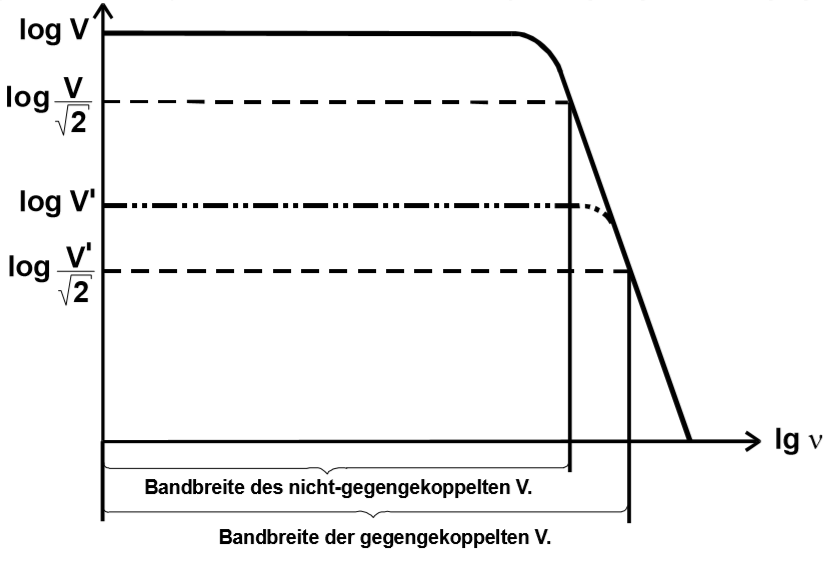
\includegraphics[width=0.55\textwidth]{bilder/bandbreite.png}
    \caption{Exemplarisches Auftragen des Logarithmus der Verstärkung gegen den Logarithmus der Frequenz des Eingangssignals. Es zeigt sich ein Frequenzband, in dem ein linearer Zusammenhang auftritt \cite{anleitung}.}
    \label{abb:bandbreite}
  \end{figure}

\subsubsection{Umkehr-Integrator}
Über einen Kondensator $C$, der in den Rückkopplungskreis eingebaut wird, kann das Eingangssignal integriert werden. Zu sehen ist eine solche Integrator-Schaltung in Abbildung \ref{integrator}.

\begin{figure}[H]
  \centering
  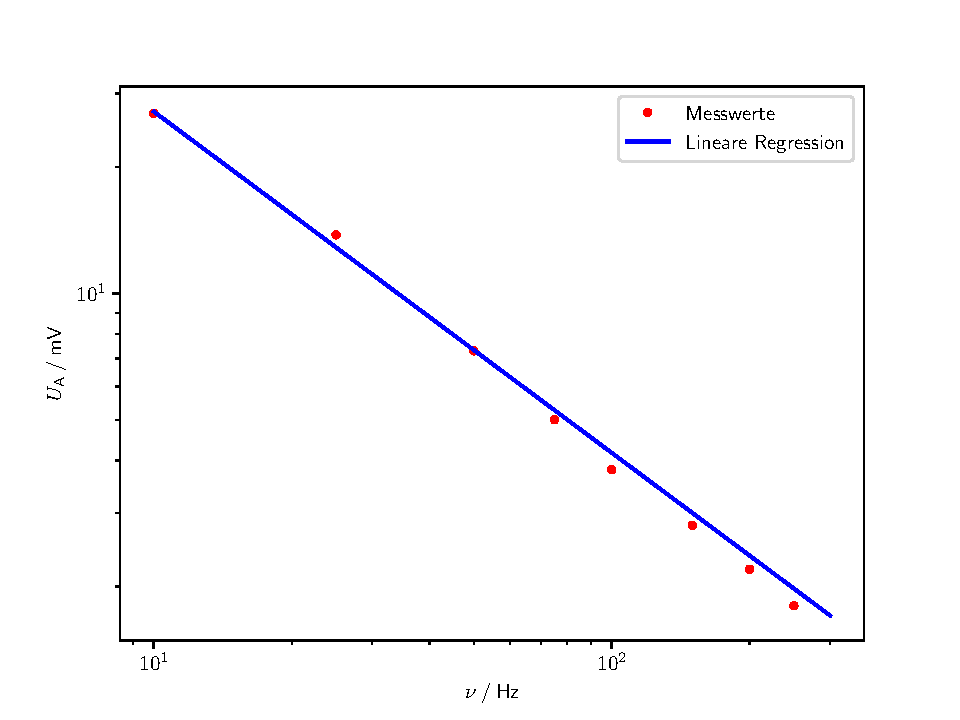
\includegraphics[width=0.45\textwidth]{bilder/integrator.png}
  \caption{Schematische Darstellung eines Umkehr-Integrators \cite{anleitung}.}
  \label{integrator}
\end{figure}

Aufgestellt werden kann die Beziehung
\begin{equation}
  \int_{}^{} I_\text{C} \ dt=CU_\text{A}\,,
\end{equation}
die die exponentielle Kennlinie des Kondensators berücksichtigt.
Für den Knoten A lässt sich mit der Knotenregel
\begin{equation}
  U_\text{A}=-\frac{1}{RC}\int_{}^{} U_1(t) \ dt
\end{equation}
aufstellen. Gibt man ein sinusförmiges Eingangssignal $U_1=U_0\sin(\omega t)$ auf die Schaltung, folgt $U_\text{A}=\frac{U_0}{\omega RC}\cos(\omega t)$ als integriertes Ausgangssignal $U_\text{A}$. Erkennen lässt sich ebenso die Antiproportionalität der Ausgangsspannung zur Frequenz $\omega$.
\subsubsection{Umkehr-Differentiator}
Werden Widerstand und Kondensator in der Schaltung des Umkehr-Integrators vertauscht, so wird eine Umkehr-Differentiator-Schaltung, wie in Abbildung \ref{differentiator} gezeigt ist, erstellt.

\begin{figure}[H]
  \centering
  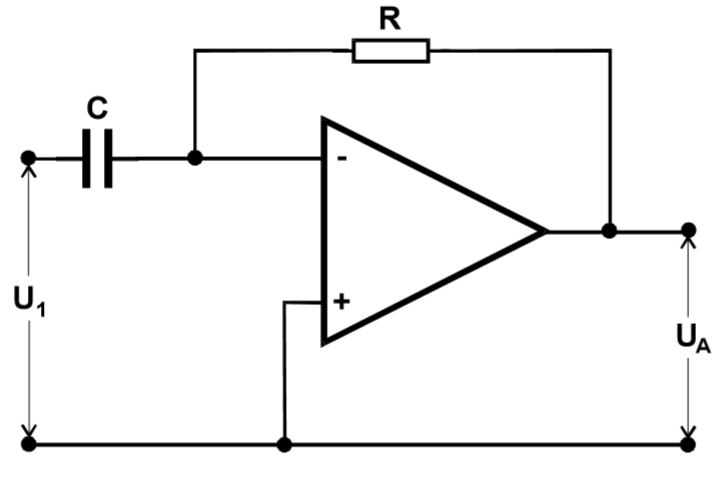
\includegraphics[width=0.45\textwidth]{bilder/differentiator.png}
  \caption{Schematische Darstellung eines Umkehr-Differentiators \cite{anleitung}.}
  \label{differentiator}
\end{figure}

Für einen solchen lässt sich die Beziehung
\begin{equation}
  U_\text{A}=-RC\frac{dU_1}{dt}
\end{equation}
für die Ausgangsspannung herleiten. Wird wiederum eine Sinusspannung als Eingangssignal $U_1=U_0\sin(\omega t)$ verwendet, folgt somit $U_\text{A}=-\omega RCU_0\cos(\omega t)$. Hierbei ist die Amplitude der Ausgangsspannung direkt proportional zu der Kreisfrequenz $\omega$.
\subsection{Schmitt-Trigger}
Der Schmitt-Trigger ist ein prominentes Beispiel einer Schaltung, die mit einer sogenannten Mitkopplung arbeitet. Wie in Abbildung \ref{schmitti} zu sehen ist, wird das Ausgangssignal auf den nicht-invertierenden Eingang zurückgekoppelt. Hierbei soll das Ausgangssignal dem Eingang nicht entgegenwirken, sondern diesen verstärken.
Im Gegensatz zu zum Beispiel Transistoren besitzen Schmitt-Trigger zwei klar definierte Werte für die Schaltschwelle, bei der der Zustand umklappt. Ein Schmitt-Trigger kann somit als Sinus-Rechteck-Wandler arbeiten. Wird ein Sinussignal in den Eingang gegeben, so steigt die Spannung am Schmitt-Trigger zunächst an. Das geschieht solange, bis die Spannung einen kritischen Wert, dem der Schaltschwelle erreicht hat. Der Ausgangsspannungswert kippt von einem Zustand in den anderen. Wird der Wert der zweiten Schaltschwelle erreicht, ändert sich die Ausgangsspannung wiederum schlagartig zu dem alten Wert.
Dies ermöglicht der Schaltung die Eigenschaften eines Schalters.
Es ergibt sich eine rechteckige Form der Hysterese mit klar definierten Schaltwerten, siehe Abbildung \ref{abb:hysterese}.
Der Schwellenwert ergibt sich zu
\begin{equation}
U_+=\frac{R_1}{R_\text{p}}U_\text{B}\,.
\label{eq:schmitti}
\end{equation}
Wird der Wert $U_+$ überschritten, springt $U_A$ auf den Wert $+U_B$; ebenfalls springt $U_\text{A}$ auf den Wert $-U_\text{B}$, wenn der Schwellenwert von $-\frac{R_1}{R_\text{p}}U_\text{B}$ unterschritten wird.

\begin{figure}[H]
  \centering
  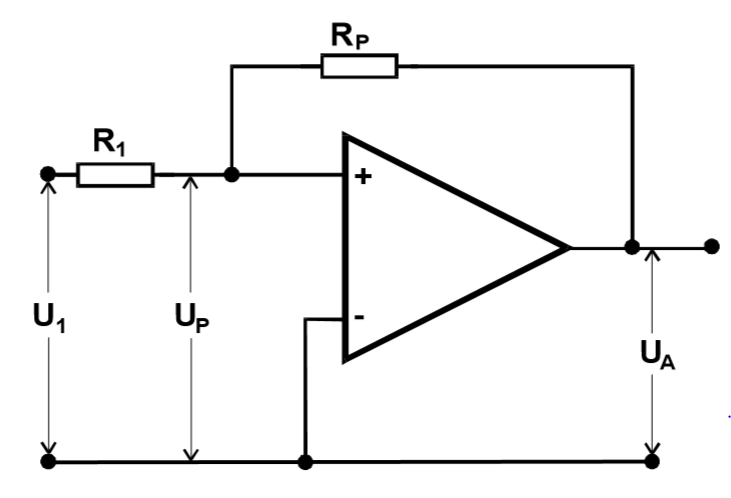
\includegraphics[width=0.45\textwidth]{bilder/schmitti.png}
  \caption{Schematische Darstellung eines Schmitt-Triggers mit den Mitkopplungswiderständen $R_1$ und $R_\text{p}$ \cite{anleitung}.}
  \label{schmitti}
\end{figure}
\begin{figure}[H]
  \centering
  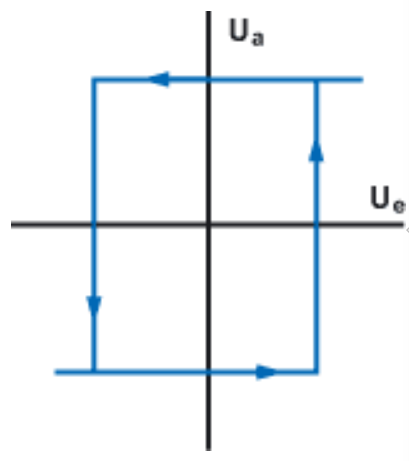
\includegraphics[width=0.30\textwidth]{bilder/hysterese.png}
  \caption{Schematische Darstellung der rechteckigen Schalthysterese eines Schmitt-Triggers \cite{hysterese}.}
  \label{abb:hysterese}
\end{figure}
